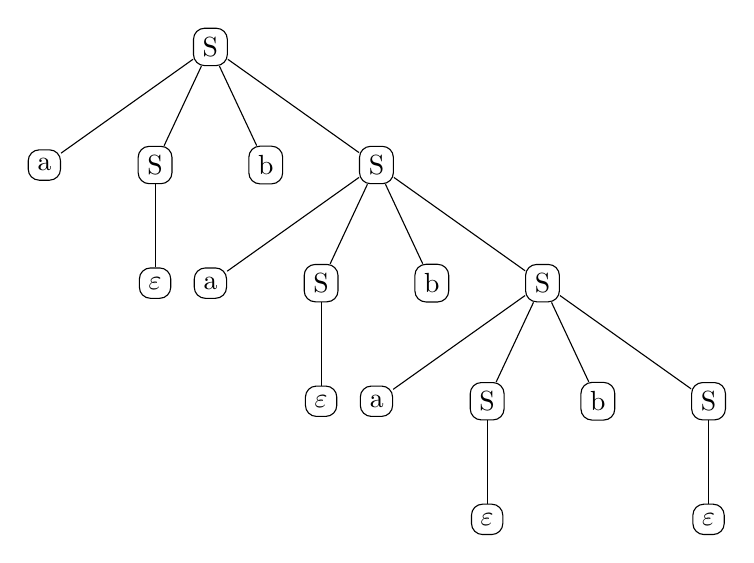
\begin{tikzpicture}[sibling distance=4em,
  every node/.style = {shape=rectangle, rounded corners,
    draw, align=center}]]
  \node {S}
    child { node {a} }
    child { node {S}
      child { node {$\varepsilon$}}
    }
    child { node {b} }
    child { node {S}
      child {node {a}}
      child { node {S}
        child { node {$\varepsilon$}}
      }
      child { node {b} }
      child { node {S}
        child {node {a}}
        child {node {S}
          child {node {$\varepsilon$}}
        }
        child {node {b}}
        child {node {S}
          child {node {$\varepsilon$}}
        }
      }
    };
\end{tikzpicture}